    \begin{figure}[!htbp]
        \centering
        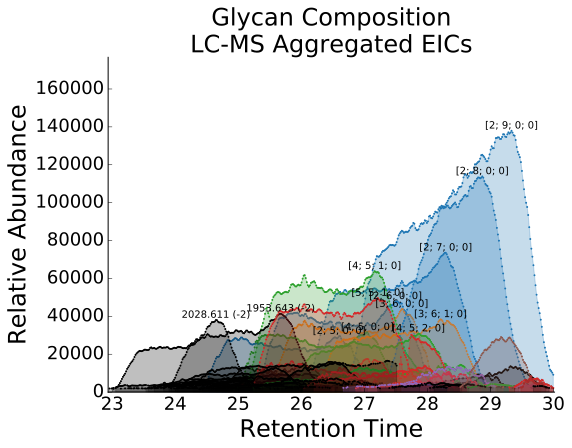
\includegraphics[width=0.45\textwidth,valign=t]{figure/phil_bs_chromatograms.pdf}
        \includegraphics[width=0.45\textwidth,valign=t]{figure/phil_bs_abundances.pdf}
        \caption{\textit{20141101-04-Phil-BS} Glycan Relative Abundances}
        \label{fig:phil_bs_aggregated_eics}
    \end{figure}

    \begin{table}
        \begin{minipage}[t]{0.25\linewidth}
            \vspace{0pt}
            (a)
            \centering
            
    \begin{tabular}{l | c}
        Group & $\tau$ \\
        \hline
        high-mannose & 1.86 \\
        hybrid & 1.50 \\
        bi-antennary & 0.00 \\
        asialo-bi-antennary & 1.70 \\
        tri-antennary & 0.00 \\
        asialo-tri-antennary & 0.94 \\
        tetra-antennary & 0.00 \\
        asialo-tetra-antennary & 0.89 \\
        penta-antennary & 0.00 \\
        asialo-penta-antennary & 0.61 \\
    \end{tabular}
    
            
        \end{minipage}
        \hspace{1cm}
        \begin{minipage}[t]{0.55\linewidth}
            \vspace{0pt}
            (b)
            \centering
            
    \begin{footnotesize}
    \begin{tabular}{l|p{2cm} p{2cm}}
Glycan Compostion &  Unregularized Score &  Regularized Score \\
\hline
\{Hex:5; HexNAc:2\}                  &                18.44 &              18.03 \\
\{Hex:6; HexNAc:2\}                  &                17.74 &              17.53 \\
\{Hex:7; HexNAc:2\}                  &                17.94 &              17.64 \\
\{Hex:8; HexNAc:2\}                  &                19.02 &              18.64 \\
\{Hex:9; HexNAc:2\}                  &                19.91 &              19.37 \\
\{Fuc:1; Hex:4; HexNAc:3\}           &                10.74 &              10.40 \\
\{Hex:5; HexNAc:3\}                  &                11.95 &              11.90 \\
\{Hex:5; HexNAc:3; Neu5Ac:1\}        &                 7.71 &               7.68 \\
\{Hex:6; HexNAc:3\}                  &                19.15 &              18.62 \\
\{Fuc:1; Hex:6; HexNAc:3\}           &                17.20 &              16.62 \\
\{Hex:7; HexNAc:3; Neu5Ac:1\}        &                 8.19 &               7.98 \\
\{Fuc:1; Hex:4; HexNAc:4; Neu5Ac:1\} &                 9.02 &               8.66 \\
\{Hex:5; HexNAc:4\}                  &                15.62 &              15.31 \\
\{Hex:5; HexNAc:4; Neu5Ac:1\}        &                11.41 &              11.05 \\
\{Fuc:1; Hex:5; HexNAc:4\}           &                17.64 &              17.15 \\
\{Fuc:1; Hex:5; HexNAc:4; Neu5Ac:1\} &                 7.95 &               7.87 \\
\{Fuc:2; Hex:5; HexNAc:4\}           &                16.33 &              15.72 \\
\{Fuc:3; Hex:5; HexNAc:4\}           &                11.08 &              10.83 \\
\{Fuc:1; Hex:6; HexNAc:4\}           &                12.31 &              12.11 \\
\{Hex:7; HexNAc:4\}                  &                11.97 &              11.58 \\
\{Hex:8; HexNAc:4; Neu5Ac:2\}        &                 6.75 &               6.50 \\
\{Fuc:1; Hex:4; HexNAc:5\}           &                12.16 &              11.74 \\
\{Hex:5; HexNAc:5\}                  &                17.18 &              16.63 \\
\{Fuc:1; Hex:5; HexNAc:5\}           &                17.37 &              16.80 \\
\{Fuc:2; Hex:5; HexNAc:5\}           &                 8.08 &               8.06 \\
\{Fuc:3; Hex:5; HexNAc:5\}           &                 7.51 &               7.33 \\
\{Hex:6; HexNAc:5\}                  &                10.03 &               9.89 \\
\{Fuc:1; Hex:6; HexNAc:5\}           &                11.89 &              11.63 \\
\{Fuc:2; Hex:6; HexNAc:5\}           &                 8.99 &               8.78 \\
\{Fuc:3; Hex:6; HexNAc:5\}           &                 8.19 &               7.92 \\
\{Hex:9; HexNAc:5; Neu5Ac:2\}        &                11.40 &              10.72 \\
\{Fuc:1; Hex:6; HexNAc:6\}           &                 7.79 &               7.59 \\
\{Fuc:1; Hex:7; HexNAc:6\}           &                 9.13 &               8.81 \\
\{Fuc:2; Hex:7; HexNAc:6\}           &                 7.39 &               7.20 \\
\{Fuc:3; Hex:7; HexNAc:6\}           &                 7.46 &               7.15 \\
\{Fuc:1; Hex:8; HexNAc:7\}           &                17.25 &              16.39 \\
\{Fuc:2; Hex:8; HexNAc:7\}           &                15.20 &              14.46 \\
\{Hex:3; HexNAc:8; Neu5Ac:4\}        &                10.11 &               9.56 \\
\{Fuc:1; Hex:9; HexNAc:8\}           &                13.44 &              12.70 \\
\end{tabular}

    \end{footnotesize}
    
        \end{minipage}
        \caption{
                 Search Results for \textit{20141101-04-Phil-BS}.
                 (a) Estimated $\mathbf{\tau}$ for grid with ${\hat \gamma} = 15.74699$.
                 (b) Scores For Identified Glycans of grid with ${\hat \lambda} = 0.01$.}
        \label{tbl:phil_bs_score_table}
    \end{table}
